\documentclass{article}
\usepackage[margin=1in]{geometry}
\usepackage{fancyvrb}
\usepackage{multicol}
\usepackage{hyperref}
\usepackage{amsmath}
\usepackage{amsfonts}

\usepackage[listings]{tcolorbox}

\definecolor{codegreen}{rgb}{0,0.6,0}
\definecolor{codegray}{rgb}{0.5,0.5,0.5}
\definecolor{codepurple}{rgb}{0.58,0,0.82}
\definecolor{backcolour}{rgb}{0.95,0.95,0.92}

\lstdefinestyle{mystyle}{
    language=Python,
    backgroundcolor=\color{backcolour},   
    commentstyle=\color{codegreen},
    keywordstyle=\color{magenta},
    numberstyle=\tiny\color{codegray},
    stringstyle=\color{codepurple},
    basicstyle=\ttfamily\footnotesize,
    breakatwhitespace=false,         
    breaklines=true,                 
    captionpos=b,                    
    keepspaces=true,                 
    numbers=left,                    
    numbersep=5pt,                  
    showspaces=false,                
    showstringspaces=false,
    showtabs=false,                  
    tabsize=2,
    escapechar=|,
    frame=single
}

\lstset{style=mystyle}

\newcommand{\showfig}[2]{
\noindent\includegraphics[width=\textwidth]{#1}
\centerline{#1}
}
\newcommand{\bi}{\begin{itemize}}
\newcommand{\li}{\item}
\newcommand{\ei}{\end{itemize}}

\usepackage{graphicx}
\usepackage{hyperref,fancyvrb,amsmath}
\usepackage{tikz}
\usepackage{tikz-qtree}

\newcommand{\mydot}[1]{\draw[fill] (#1) circle (0.1);}

\newcommand{\set}[1]{\ensuremath{\{#1\}}}

\title{Maze Solver}
\author{CSCI112, Lab 10}

\begin{document}

\maketitle
\centerline{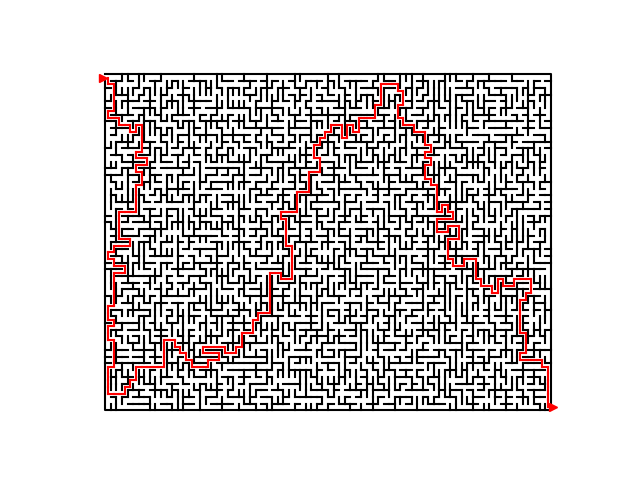
\includegraphics[scale=1]{Figure_1}}

\begin{description}

\item[File names:]  Names of files, functions, and variables, 
when specified,
must be EXACTLY as specified.  This includes simple mistakes such
as capitalization.

\item[Individual work:]  All work must be your own.  Do not share
code with anyone other than the instructor and teaching assistants.
This includes looking over shoulders at screens with the code open.
You may discuss ideas, algorithms, approaches, {\em etc.} with
other students but NEVER actual code.  Do not use code
written by anyone else, in the class or from the internet.

\item[Documentation:] Each file should begin with a docstring
that includes your name, the class number and name, the lab
number, and  
a short description of the lab, as well as documentation pertinent
to that particular file.

  
\item[Solving a maze:]  Now that you know how to generate a maze,
solving a maze with depth-first search is easy!

In your maze generation program, you found the walls of the maze
by repeatedly joining two adjacent cells, putting a ``door'' between
them and erasing the wall.  You saved the walls so you could draw 
them.

Now we want to save all the doors.  This will be a list of all pairs
of cells that are connected to each other by a door.  These
pairs form the edges of a graph.  Transform
this list of pairs into an adjacency list representation of the graph,
which can be a dictionary with cells as keys and lists of other
cells that are connected to them.

If there is a door between cell $a$ and cell $b$, be sure to 
add an edge from $a$ to $b$ and one from $b$ to $a$!

\item[Depth first search:]  You can now use a simple stack
to search for a solution to the maze.  When each node is
placed on the ``gray'' stack, you can record its predecessor
in another dictionary.  The start node has predecessor {\tt None}.

When the end node has a predecessor, you can stop
the search!

Do not use recursion.  Use a stack for depth-first search
so that depth-first, breadth-first, and next week's ``best-first''
searches all look the same, except for the order of
the gray nodes in the data structure.

\item[Random seed:] If you want to draw the same maze
every time, set the random seed to the same value before
shuffling the edges:  {\tt random.seed(1234)}, for example. 
\item[Drawing the solution:]
This predecessor list will enable
you to draw the solution by starting at the end point, and drawing
a line from predecessor to predecessor, until there are no more
predecessors.

Feel free to use my drawing code.  I've modified the {\tt drawMaze}
routine to facilitate drawing the solution path.  (It also helps with
some ``off by one'' problems some students had with my original
drawing routine.)  

After both of these routines have been called, call the {\tt plt.show()}
routine to show the drawing.

\begin{lstlisting}
def drawMaze(walls, mazeSize):
    nrows, ncols = mazeSize
    fig, ax = plt.subplots()
    ax.axis("off")
    # draw outer box
    lo = -0.5
    hix = ncols-0.5
    hiy = nrows-0.5
    plt.plot((lo, lo, hix), (hiy-1, lo, lo), color='black')
    plt.plot((lo, hix, hix), (hiy, hiy, lo+1), color='black')
    # draw walls
    for wall in walls:
        a,b = wall
        y1,x1 = a
        y2,x2 = b
        if x1 == x2:
            y = (y1+y2)*0.5
            plt.plot((x1-0.5,x1+0.5), (y,y),  color='black')
        else:
            x = (x1+x2)*0.5
            plt.plot((x,x),(y1-0.5,y1+0.5),  color='black')
            
def drawPath(predecessors, mazeSize):
    nrows, ncols = mazeSize
    pos = (0, ncols-1)
    while predecessors[pos] is not None:
        y1,x1 = pos
        y2,x2 = predecessors[pos]
        plt.plot((x1,x2), (y1,y2), color='red')
        pos = predecessors[pos]
    plt.plot((ncols),(0), color='red', marker='>')
    plt.plot((-1), (nrows-1) ,color='red', marker='>')
\end{lstlisting}

\end{description}
\end{document}
